\documentclass[12pt, a4paper]{article}
% \usepackage{ctex}
\usepackage[margin=1in]{geometry} 
\usepackage{amsmath,amsthm,amssymb}
\usepackage{bm}
\usepackage{cases}
\usepackage{graphicx}
\usepackage{subfig}
\usepackage{hyperref}
\usepackage{amsfonts}
\usepackage{authblk}
\usepackage{mathrsfs}
\newcommand{\E}{\mathbb{E}}
\newcommand{\R}{\mathbb{R}}
\newcommand{\N}{\mathcal{N}}
\hypersetup{hidelinks}
\title{PRML Note\\C08 Graphical Models}
\author{Yang Zhao}
\affil{Department of Automation, Tsinghua University}
\date{}

\begin{document}
    \maketitle
    \begin{itemize}
        \item The properties of \textit{probabilistic graphical models}\begin{enumerate}
            \item Provide a simple way to visualize the structure of a probabilistic model
            and can be used to design and motivate new models.
            \item Insights into the properties of the model, including conditional independence
            properties, can be obtained by inspection of the graph. 
            \item Complex computations, required to perform inference and learning in spphisticated
            models, can be expressed in terms of graphical manipulations, in which underlying 
            mathematical expressions are carried along implicitly.
        \end{enumerate}
        \item The graph comprises vertices connected by edges, where the vertices represents a 
        random variable and the edges express probabilistic relationships between the variables.
        \item The categories of the graphical models\begin{enumerate}
            \item Bayesian networks: directed graphical models. 
            \item Markov random fields: undirected graphical models.
            \item factor graph: be used to do the inference.
        \end{enumerate}
        \item Graph terminology: a graph $G=(V,E)$ can be represented by adjacency matrix, in which
        we write $\mathbf{L}(s,t)=1$ if $(s,t)\in E$. We say the graph is undirected if $\mathbf{L}
        =\mathbf{L}^T$, otherwise it is directed. We usually assume $\mathbf{L}(s,s)=0$ which means
        there are no self loops.\begin{enumerate}
            \item \textit{Parent}: For a directed graph, the parents of a node is the set of all 
            nodes that feed into it: $Pa(s)\triangleq\{t:\mathbf{L}(t,s)=1\}$. 
            \item \textit{Child}: For a directed graph, the children of a node is the set of all 
            nodes that feed out of it: $Ch(s)\triangleq\{t:\mathbf{L}(s,t)=1\}$.
            \item \textit{Family}: For a directed graph, the family of a node is the node and its 
            parents, $Fam(s)=\{ s\}\cup Pa{s}$.
            \item \textit{Root}: For a directed graph, a root is a node with no parents.
            \item \textit{Leaf}: For a directed graph, a leaf is a node with no children.
            \item \textit{Ancestors}: For a directed graph, the ancestors are the parents, grand-
            parents, etc of a node.
            \item \textit{Descendants}: For a directed graph, the descendants are the children, 
            grand-children, etc of a node.
            \item \textit{Neighbors}: For any graph, we define the neighbors of a node as the set
            of all immediately connected nodes.
            \item \textit{Degree}: The degree of a node is the number of neighbors. For directed
            graphs, we speak of the in-degree and out-degree, which count the number of parents
            and children.
            \item \textit{Cycle or loop}: For any graph, we define a cycle or loop to be a series
            of nodes such that we can get back to where we started.
            \item \textit{DAG}: A directed acyclic graph is a directed graph with no directed
            cycles.
            \item \textit{Topological ordering}: For a DAG, a topological ordering or total ordering
            is a numbering of the noders such that parents have lower numbers than their children.
            \item \textit{Path or trail}: A path or trail $s\leadsto t$ is a series of directed 
            edges leading from $s$ to $t$.
            \item \textit{Tree}: An undirected tree is an undirected graph with no cycles. A directed
            tree is a DAG in which there are no directed cycles. If we allow a node to have multiple
            parents, we call it a polytree.
            \item \textit{Forest}: A set of trees.
            \item \textit{Subgraph}: A subgraph $G_A$ is the graph created by using the nodes in A
            and their corresponding edges, $G_A=(V_A,E_A)$.
            \item \textit{Clique}: For an undirected graph, a clique is a set of nodes that are all 
            neighbors of each other. 
        \end{enumerate}
    \end{itemize}
    
    \section{Bayesian Networks}
    \begin{itemize}
        \item For a graph with $K$ nodes, the joint distribution is given by \begin{equation*}
            p(\bm{x})=\prod_{k=1}^Kp(x_k|Pa(x_k))
        \end{equation*}
        This key equation expresses the \textit{factorization} properties of the joint 
        distribution for a directed graphical model.
        \item Three cases of 3-node graph, which is shown as the figure \ref{fig:threecases}.
        \begin{itemize}
            \item For figure \ref{fig_first_case}, if node $c$ is observed, node $a$ is independent 
            with node $b$.
            \begin{equation*}
                p(a,b|c)=p(a|c)p(b|c)
            \end{equation*}
            \item For figure \ref{fig_second_case}, if node $c$ is observed, node $a$ is independent
            with node $b$.
            \begin{equation*}
                p(a,b|c)=p(a|c)p(b|c)
            \end{equation*}
            \item For figure \ref{fig_third_case}, if node $c$ isn't observed, 
            node $a$ is independent with node $b$. This case is also called the \textit{v-structure}.
            \begin{equation*}
                p(a,b|c)\neq p(a|c)p(b|c)
            \end{equation*}
        \end{itemize}
        \begin{figure}[htbp]
            \centering
            \subfloat[]{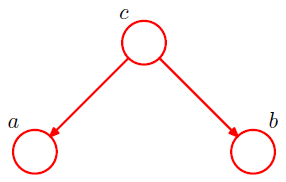
\includegraphics[width=2in]{figures/tail2tail.PNG}
            \label{fig_first_case}}
            \hfil
            \subfloat[]{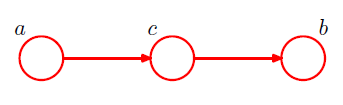
\includegraphics[width=2in]{figures/head2tail.PNG}
            \label{fig_second_case}}
            \hfil
            \subfloat[]{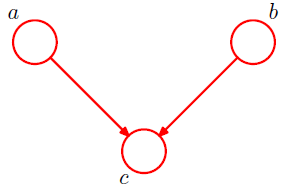
\includegraphics[width=2in]{figures/head2head.PNG}
            \label{fig_third_case}}
            \caption{Three cases of 3-node graphs. For the figure \ref{fig_first_case}, the node $c$
            is said to be tail-to-tail with respect to the path from node $a$ to $b$. 
            For the figure \ref{fig_second_case}, the node $c$
            is said to be head-to-tail with respect to the path from node $a$ to $b$.
            For the figure \ref{fig_third_case}, the node $c$
            is said to be head-to-head with respect to the path from node $a$ to $b$.}
            \label{fig:threecases}
        \end{figure}
        \item \textit{The blocked path}. Any path is said to be blocked if it includes a node such that 
        either \begin{itemize}
            \item[a] the arrows on the path meet either head-to-tail or tail-to-tail at the node, and
            the node is observed, or
            \item[b] the arrows meet head-to-head at the node, and neither the node, nor any of its 
            descendants, is observed.  
        \end{itemize}
        \item \textit{D-separation}. Consider a general directed graph in which $A$, $B$ and $C$ are 
        arbitrary nonintersecting sets of nodes. If all paths from any node in $A$ to any node in 
        $B$ are blocked, then $A$ is said to be D-separation from $B$ by $C$ and we have 
        $A\perp B|C$.
        \item \textit{Markov blanket}. For directed graph, the Markov blanket of a node comprises the set of 
        parents, children and co-parents of the node. Denote the Markov blanket of a node $x_i$ with 
        $Mb(x_i)$ and we have $x_k\perp x_i|Mb(x_i)$, where $x_k$ is any node except $x_i$ and 
        $Mb(x_i)$.
    \end{itemize}

    \section{Markov Random Fields}
    \begin{itemize}
        \item A Markov Random Field, also known as a Markov network or an undirected graphical model, 
        has a set of nodes and undirected edges.
        \item The Markov blanket of an undirected graph is the set of all neighbouring nodes because 
        a node will be conditionally independent of all other nodes conditioned only on the 
        neighbouring nodes.
        \item Factorization properties of Markov random fields. Let us denote a clique by $C$ and the 
        set of variables in that clique by $\bm{x}_C$. Then the joint distribution is written as a 
        product of potential functions $\psi_C(\bm{x}_C)$ over the maximal cliques of the graph
        \begin{equation*}
            p(\bm{x})=\frac{1}{Z}\prod_C\psi_C(\bm{x}_C)
        \end{equation*}
        where the $Z$, called the partition function, is a normalization constant and is given by 
        \begin{equation*}
            Z=\sum_{\bm{x}}\prod_C\psi_C(\bm{x}_C)
        \end{equation*}
        \item The presence of the normalization constant is one of the major limitations of undirected 
        graphs. The partition function is needed for parameter learning because it will be a function of 
        any parameters that govern the potential functions $\psi_C(\bm{x}_C)$.
        \item It is convenient to express them as exponentials, so that
        \begin{equation*}
            \psi_C(\bm{x}_C)=exp\{-E(\bm{x}_C)\}
        \end{equation*}
        where $E(\bm{x}_C)$ is called an energy function, and the exponential representation is called the 
        Boltzmann distribution. 
    \end{itemize}
    \section{Inference in Graphical Models}
    \begin{itemize}
        \item \textit{Inference}. The task of inference is that we know all the parameters of the model and
        caculate the marginal probability and the conditional probability. 
    \end{itemize}
\end{document}